
\begin{sstTitleBox}{
		Discrete-Time Optimal Control Problem
	}
	\begin{sstOnlyFrame}
		\textbf{Cost Function}
		\vspace{-3mm}
		\begin{equation}
			J(x_0,U)= \sum_{i=0}^{N-1} l(x_i,u_i) + l_f(x_N)
		\end{equation}
		% \vspace{-2mm}
		\begin{minipage}[t]{0.25\linewidth}
			\textbf{Stage Cost}
			$l_f(x_i,u_i)$
			\textbf{Terminal Cost}
			$l_f(x_N)$
		\end{minipage}
		\begin{minipage}[t]{0.59\linewidth}
			\vspace{-5.5mm}
			\begin{align*}
				\textbf{Constraints}                      \\
				x_{i+1}    & = g(x_i,u_i)                 \\
				x_0        & = x(k)                       \\
				h(x_i,u_i) & \le 0 \quad\text{(optional)}
			\end{align*}
		\end{minipage}
	\end{sstOnlyFrame}
\end{sstTitleBox}

\subsection{Unconstrained Finite Horizon Control Problem}

\begin{sstTitleBox}
	{Linear Quadratic Optimal Control}
	\begin{sstOnlyFrame}
		\textbf{Cost Function}
		\vspace{-3mm}
		\begin{equation}
			J^\star(x(0)) := \min_U
			\sum_{i=0}^{N-1}
			x_i^\top Q x_i + u_i^\top R u_i
			+x_N^\top P x_N
			\label{oc:lq-oc}
		\end{equation}

		\vspace{-2mm}
		\begin{minipage}[t]{0.33\linewidth}
			\textbf{Terminal weight}

			$P\succeq0$ symetric

			\textbf{State weight}

			$Q\succeq0$ symetric

			\textbf{Input weight}

			$R\succ0$ symetric
		\end{minipage}
		\begin{minipage}[t]{0.49\linewidth}
			\textbf{Constraints}

			No input or state constraints!
			\[
				x(k+1)=Ax_k+Bu_k
			\]
			Only dynamics matter.
		\end{minipage}

	\end{sstOnlyFrame}
\end{sstTitleBox}

\subsubsection{Batch Approach}

express cost function in terms of $x(0)$ and input sequence $U$
%
\[ \begin{bmatrix}
		x_0    \\
		x_1    \\
		\vdots \\
		x_N
	\end{bmatrix}
	=
	\begin{bmatrix}
		\mathbb{I} \\
		A          \\
		\vdots     \\
		A^N
	\end{bmatrix}
	x(0) +
	\begin{bmatrix}
		0        & \cdots & 0 \\
		B        & 0      & 0 \\
		AB       & B      & 0 \\
		\vdots   & \ddots & 0 \\
		A^{N-1}B & \cdots & B
	\end{bmatrix}
	\begin{bmatrix}
		u_0    \\
		u_1    \\
		\vdots \\
		u_{N-1}
	\end{bmatrix} \]
%
$X:=\mathcal{S}^x x(0) + \mathcal{S}^u U$
\quad
$J(x(0),U) =
	X^\top \overline{Q}X
	+ U^\top \overline{R}U$

$\overline{Q} := \mathop{\mathrm{blockdiag}}(Q,\dots, Q,P)$
\quad
$\overline{R} := \mathop{\mathrm{blockdiag}}(R,\dots, R)$

\textbf{Optimal Input}
set $\nabla_UJ(x(0),U)=2HU+2F^\top x(0)=0$
\[ U^\star(x(0)) =
	- \bigl(
	\underbrace{
			(\mathcal{S}^u)^\top \overline{Q} \mathcal{S}^u + \overline{R}
		}_{H\text{(Hessian)}^{-1}}
	\bigr)
	\underbrace{
		(\mathcal{S}^u)^\top \overline{Q}\mathcal{S}^x
	}_ {F^\top}
	x(0)
\]

\textbf{Optimal Cost}
$(x_0=x(0))$
\[
	\scriptstyle
	J^\star(x_0) = x_0^\top (
	\mathcal{S}_x^\top \overline{Q} \mathcal{S}_x
	- \mathcal{S}_x^\top \overline{Q} \mathcal{S}_u
	(\mathcal{S}_u^\top \overline{Q} \mathcal{S}_u
	+ \overline{R})^{-1}
	\mathcal{S}_u^\top \overline{Q} \mathcal{S}_x
	)x_0
\]

\subsubsection{Recursive Approach}

use dynamic programming to solve problem backwards from $N$
%
\begin{align*}
	J_j^\star(x(j)) :=
	\min_{U_{j\to N}} & x_N^\top P x_N \!+
	\sum_{i=j}^{N-1}x_i^\top Q x_i + u_i^\top R u_i
\end{align*}
%
\begin{minipage}[t]{0.64\linewidth}
	\textbf{From Principle Of Optimality}
	\[
		J_j^\star(x_j) =
		\min_{u_j} I(x_i,u_i) + J_{j+1}^\star(x_{j+1})
	\]
\end{minipage}
\begin{minipage}[t]{0.32\linewidth}
	\textbf{Optimal Cost-To-Go}
	\[
		J_i^\star(x_i) = x_i^\top P_i x_i
	\]
\end{minipage}
%
\textbf{Optimal Control Policy}
use Riccatti
\[
	u_i^\star = F_i x_i =
	-(B^\top P_{i+1}B + R)^{-1}
	B^\top P_{i+1} A \cdot x(i)
\]

\subsubsection{Comparison of Batch and Recursive Approach}

Dynamic programming yields \textbf{feedback policies}
$u_i^\star = F_i x_i$ depending on each $x_i$.
Batch optimization returns sequence $U^\star(x(0))$
of \textbf{numeric values} depending only on x(0),

\subsection{Infinite Horizon Control Problem}

\begin{sstTitleBox}{
		Linear Quadratic Regulator
	}
	\begin{sstOnlyFrame}
		\textbf{Cost Function}
		\vspace{-3mm}
		\begin{equation}
			J_\infty^\star(x(k)) =
			\min_{u(\cdot)} \sum_{i=0}^\infty
			x_i^\top Q x_i + u_i^\top R u_i                                   \\
		\end{equation}

		\vspace{-5mm}
		\begin{minipage}[t]{0.67\linewidth}
			\begin{align*}
				 & \textbf{Constraints}
				 & x_{i+1}                & = Ax_i + Bu_i
				\\
				 &                        & x_0             & = x(k)
				\\ \\
				 & \textbf{Optimal Input}
				 & u^\star(k)             & = F_\infty x(k)
				 & \text{(use Riccatti)}
			\end{align*}
		\end{minipage}
		\begin{align*}
			F_\infty x(k)		=           - (B^\top P_\infty B + R)^{-1}
			B^\top P_\infty A x(k)
		\end{align*}
	\end{sstOnlyFrame}

	\begin{sstOnlyFrame}
		\begin{lemma}[Lyapunov function for LQR]
			If $(A,B)$ is stabilizable
			and $Q,R \succ 0$ then
			$J^\star(x) = x^\top P_\infty x$
			is a \ssthl{ Lyapunov function }
			for the system $x^+ = (A+BF_\infty)x$
			where $F_\infty$ is the constant feedback matrix
			and $P_\infty \succ 0$ solves the Riccatti equation..
		\end{lemma}

	\end{sstOnlyFrame}
\end{sstTitleBox}

\begin{sstTitleBox}[BrickRed]{
		Choice of P
	}
	\begin{sstOnlyFrame}[BrickRed]
		\ssthl{ 1 }
		Match the infinite solution $P_N = P_\infty$

		\ssthl{ 2 }
		Use solution of the Lyapunov Equation (\ref{lipunov:dt})
		if the system is asymptotically stable
		(otherwise P not positive definite),
		assumes no control needed after end of horizon.

		\ssthl{ 3 }
		Set $P=0$ und use instead constraint $x_{i+N}=0$
	\end{sstOnlyFrame}
\end{sstTitleBox}

\subsection{Constrained Finite Time Optimal Control Problem}

\begin{sstTitleBox}{
		CFTOC
	}
	\begin{sstOnlyFrame}
		\textbf{Cost Function} equal to
		Linear Quadratic Optimal Control (\ref{oc:lq-oc})
		% \vspace{-5mm}
		\textbf{Constraints}
		as in (\ref{oc:lq-oc})
		\ssthl{ + }
		$ x_N      \in \mathcal{X}_f$,
		$ x_{i<N}  \in \mathcal{X}$,
		$ u_i      \in \mathcal{U}$
	\end{sstOnlyFrame}

\end{sstTitleBox}

\subsubsection{Quadratic Cost CFTOC}
\[
	J(x(k)) = x_N^\top P x_N + \sum_{i=0}^{N-1}x_i^\top Q x_i + u_i R u_i
\]
\subsubsection{Goal: Transform  into QP}
\[
	\min_{z\in\mathbb{R}^n}
	\textstyle\frac{1}{2}z^\top H z + q^\top z + r
	\quad\text{s.t. }Gz\leq h,\ Az = b\]

\subsubsection{Construction of QP without Substitution}

\textbf{Idea} Keep state equations as equality constraints

\textbf{Define variable} $z =
	\begin{bmatrix}
		x_1^\top & \dots x_N^\top & u_0^\top & \dots u_{N-1}^\top
	\end{bmatrix}^\top$

\textbf{Equalities} from system dynamics
$x_{i+1} = Ax_i + Bu_i$

\[
	G_{eq} =
	\begin{bmatrix}
		\begin{smallmatrix}
			\mathbb{I}& & & \\
			-A & \mathbb{I} && \\
			&  \ddots & \ddots \\
			&&-A & \mathbb{I}
		\end{smallmatrix}
		 & \vline
		\begin{smallmatrix}
			-B \\
			& \ddots \\
			& &-B
		\end{smallmatrix}
	\end{bmatrix}
	E_{eq} =
	\begin{bsmallmatrix}
		A      \\
		0      \\
		\vdots \\
		0
	\end{bsmallmatrix}
\]

\textbf{Inequalities}
$G_{in}z \leq w_{in} + E_{in}x(k)$
for $\mathcal{X},\mathcal{U}$

\begin{minipage}[c]{0.5\linewidth}
	$\mathcal{X} = \{x \mid A_x x \le \mathcal{X}_fq b_x\}$
	$\mathcal{U}   = \{u \mid A_u u \leq b_u\}$
	$\mathcal{X}_f = \{x \mid A_f x \leq b_f\}$
\end{minipage}
\begin{minipage}[b]{0.4\linewidth}
	\[E_{in} =
		\left[
			\begin{smallmatrix}
				-A_x \\
				0 \\
				\vdots \\
				0 \\
			\end{smallmatrix}
			\right]\]
\end{minipage}
\[
	G_{in} =
	\left[
		\begin{array}{l!{\color{RoyalBlue!50}\vrule}l}
			\noalign{\arrayrulewidth=0.1mm}\arrayrulecolor{RoyalBlue!50}
			%
			\begin{smallmatrix}
				0&&&
			\end{smallmatrix}
			 &
			\begin{smallmatrix}
				0&&&
			\end{smallmatrix}
			\\ \hline
			\begin{smallmatrix}
				A_x&&&\\
				&\ddots&\\
				&&		A_x&\\
				&&&		A_f
			\end{smallmatrix}
			 &
			\begin{smallmatrix}
				0\ \ &&&\\
				&\ \ddots\\
				&&\ 0\ &\\
				&&&\ \ 0
			\end{smallmatrix}
			\\ \hline
			\begin{smallmatrix}
				0\ \ &&&\\
				&\ \ddots\\
				&&\ 0\ &\\
				&&&\ \ 0
			\end{smallmatrix}
			 &
			\begin{smallmatrix}
				A_u&&\\
				&\ddots&\\
				&&A_u&\\
				&&&A_u
			\end{smallmatrix}
		\end{array}
		\right]
	%
	w_{in} =
	\begin{bmatrix}
		\noalign{\arrayrulewidth=0.1mm}\arrayrulecolor{RoyalBlue!50}
		\begin{smallmatrix}
			b_x\\
		\end{smallmatrix}
		\\ \hline
		\begin{smallmatrix}
			b_x\\
			\vdots\\
			b_x\\
			b_f\\
		\end{smallmatrix}
		\\ \hline
		\begin{smallmatrix}
			b_u\\
			\vdots\\
			b_u\\
			b_u\\
		\end{smallmatrix}
	\end{bmatrix}
\]

\textbf{Cost Matrix} $\bar{H} = \mathrm{diag}(Q,..., Q, P, R,..., R)$

\textbf{Finally the resulting quadratic optimization problem}
\[\begin{aligned}
		J^\star(x(k)) = \min_z  \left[ z^\top \ x(k)^\top \right]
		\left[\begin{smallmatrix} \bar{H} & 0 \\ 0 & Q \end{smallmatrix}\right]
		\left[ z^\top \ x(k)^\top \right]^\top \\
		\text{s.t}
		\quad G_{in}z \leq w_{in} + E_{in}x(k)
		\quad	G_{eq}z = E_{eq}x(k)
	\end{aligned}\]

\subsubsection{Construction of QP with substitution}

\textbf{Idea} Substitute the state equations.

\textbf{Step 1} Rewrite cost  as

\[\begin{aligned}
		J(x(k)) = & U^\top HU+2x(k)^\top FU+x(k)^\top Y x(k) \\
		=         & \begin{bmatrix}
			            U^\top & x(k)^\top
		            \end{bmatrix}
		\left[\begin{smallmatrix}
				      H & F^\top \\
				      F & Y
			      \end{smallmatrix}\right]
		\begin{bmatrix}
			U^\top & x(k)^\top
		\end{bmatrix}^\top
	\end{aligned} \]

\textbf{Step 2} Rewrite constraints compaclty as $GU\le w+Ex(k)$

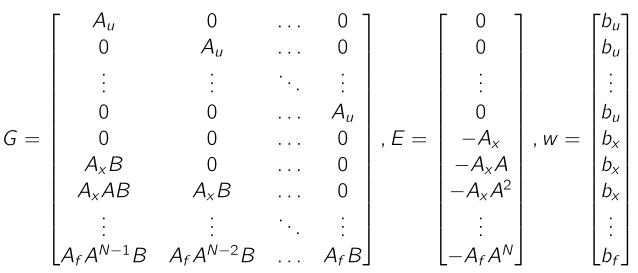
\includegraphics[width=\columnwidth]{images/qp_with_substitution.png}

\textbf{Step 3} Rewrite constrained problem as
\[\begin{aligned}
		J^\star(x(k)) = \min_U
		                       & \begin{bmatrix}
			                         U^\top & x(k)^\top
		                         \end{bmatrix}
		\left[\begin{smallmatrix}
				      H & F^\top \\
				      F & Y
			      \end{smallmatrix}\right]
		\begin{bmatrix}
			U^\top & x(k)^\top
		\end{bmatrix}^\top                          \\
		\mathrm{subj. \ to \ } & GU \leq w + Ex(k)
	\end{aligned} \]

%HACK:  transform cftoc to LP, l-norm substitution L4.p30

